\documentclass{homework}
\usepackage{ dsfont }
\usepackage[
backend=biber,
style=alphabetic,
sorting=ynt
]{biblatex}
\usepackage{csquotes} % <==================================
\addbibresource{sample.bib} %Import the bibliography file
\title{CS378 Project: Double Deep Q Learning for Frogger on Atari 2600}
\author{Dale Schandelmeier-Lynch}

\begin{document}

\maketitle
\tableofcontents
\nocite{*}
\section{Technical overview}
This project is written in Python mainly using the PyTorch and Gymnasium packages.
We've gone over PyTorch in class already, and Gymnasium is a reinforcement learning API that handles environment creation and modification.
\subsection{Installation}
Assuming you already have a working environment for PyTorch, you will only need the "gymnasium[atari]" and "gymnasium[accept-rom-license]" packages to run the notebook. Additionally the "gymnasium[other]" package is needed for the visualization at the end of the notebook. If you're using an Nvdia GPU, you may want to change the chosen GPU to 0; I was using GPU 1 because it had less usage on the remote computer I was using.
\newpage
\section{Background}
We have worked with Deep Q-networks in class, so I will assume familiarity with the subject. While Q-networks are useful for finding an optimal policy, they face an overestimation issue due to maximization bias. Q-networks take the action with the maximal estimated reward and implicitly assumes that this is an estimation of the actual maximal reward, which introduces bias. Sutton and Barto (pg. 134) concisely explains this with an example: "To see why, consider a
single state s where there are many actions a whose true values, $q(s, a)$, are all zero but
whose estimated values, $Q(s, a)$, are uncertain and thus distributed some above and some
below zero. The maximum of the true values is zero, but the maximum of the estimates
is positive, a positive bias". To avoid this, we can introduce a second network $Q_2(a)$. The first network will be used to decide an action to take, while the second network will decide the estimated value of taking said action. This "estimate will then be unbiased in the
sense that $\mathds{E}[Q_2 (A^*)] = q( A^*)$" according to Sutton and Barto (pg. 135), where $A^*$ is the maximal action chosen by our first Q-network; a proof is provided on page 8 of Hasselt and Guez's paper. We can then do things in the opposite order, with the action chosen by $Q_2$ and the estimate by $Q_1$ to update the other network. In practice with a deep double Q-network, it's easier to use the target network as our secondary network, and to update it as done normally in a deep Q-network; this what Hasselt and Guez do in their paper "Deep Reinforcement Learning with Double Q-learning" (pg. 4).
\begin{figure}[h]
\centering
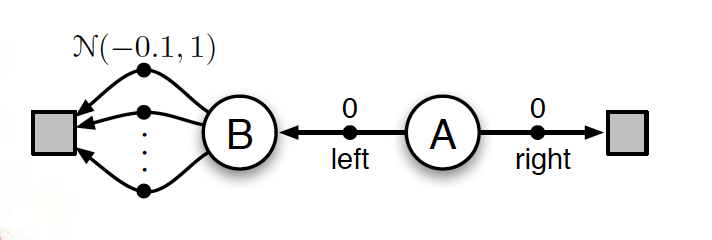
\includegraphics[width=1\linewidth]{d3B7w.png}
\caption{An example of a Markov Decision Process from \cite{Sutton_Barto_2020} where overestimation decreases performance. Although the expected value of left is $-0.1$ and of right is $0$,
a regular Q-network is likely to learn to go left, as the maximal value of the left action can be positive.}
\label{fig:1}
\end{figure}
\begin{figure}[h]
\centering
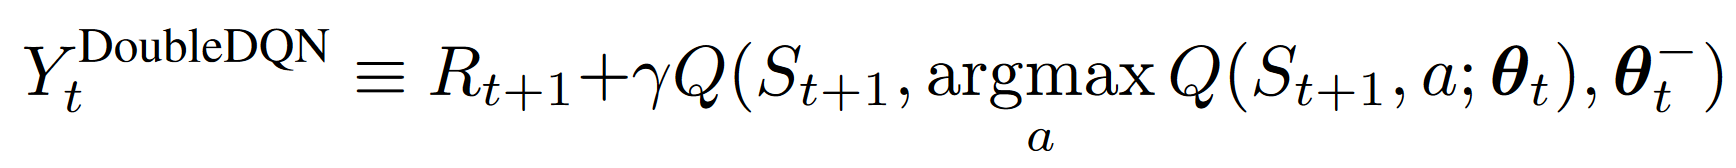
\includegraphics[width=1\linewidth]{func2.png}
\caption{The target function used by \cite{DBLP:journals/corr/HasseltGS15}. Here the online network is first used to select an action, and then the target network is used to evaluate the expected value of that action; $\theta_t$ and $\theta_t^-$ are the parameters of the online and target networks respectively.}
\label{fig:2}
\end{figure}
\newpage
\section{Implementation}
I started the project by using my finished reinforcement learning homework as a basis. I decided to do so because we were provided with code for a memory buffer and a target network, which Hasselt and Guez highly recommend (pg. 2).
Using Gymnasium provided many helpful tools to improve the quality of the environment. Rewards were directly tied to game score, which for Frogger is effective because every square moved forward rewards a point, and it would be interesting to see the network learn to do bonus objectives for bonus points. If I continued this project, I would modify the environment to penalize dying to see if this would teach the network to better preserve its lives.
\begin{figure}[h]
\centering
\begin{tabular}{|c|c|}
\hline

Successfully jumping Frogger forward& 1 point\\
Successfully jumping Frogger home& 5 points \\
Successfully jumping 5 frogs home & 100 points \\
Taking a white frog home& 20 points\\
Eating a fly& 20 points\\
Extra points for time left& 2 points \\
 & per remaining second \\
\hline
\end{tabular}
\caption{Table of ways to earn points in Frogger for Atari 2600. Every point is given a reward value of 1.}
\label{fig:3}
\end{figure}
\par Another useful feature of Gymnasium is the existence of environment wrappers, which can modify environments to improve agent performance. Atari environments come with two useful parameters, frame skip and sticky action probability. Frame skip makes the network repeat its selected action for a given amount of frames between decisions, which can improve temporal reasoning and performance. Sticky action probability gives a chance that the agent must repeat its previously selected action. Because Atari 2600 games are deterministic, this forces the agent to learn in a nondeterministic environment. Without nondeterminism, the agent can simply learn an optimal string of inputs without learning much about the network input; the resulting agent would be helpless to small changes in the environment. I used the default settings, with a frame skip of $5$ and a sticky action probability of $25\%$ In addition, the \texttt{AtariPreprocessing} wrapper adds input modification, \texttt{noop_max}, and max pooling. The input image is resized and grayscaled to an $84 \times 84 \times 1$ input into the network; reducing the size of the input speeds up both the network and its training. The parameter \texttt{noop_max} makes the agent input a no-op for a random number of frames at the start of the game, up to \texttt{noop_max}. This adds additional nondeterminism akin to sticky actions. I used the default maximum of $30$, but I realized after training that this might be insufficient. Frogger on Atari 2600 forces the player to wait at the beginning of each level for a jingle to finish playing, so its likely that these no-ops might be input when the agent couldn't do anything anyways; by the time \texttt{noop_max}is reached, the jingle hasn't ended, so the agent always gets to start the game from the exact same position. Max pooling pools over the 2 most recent observations to improve temporal logic. \par
For my network, I tried to replicate the layers provided by Sutton and Barlow on page 9. Even though I applied the same number of kernels with the same stride, I ended up with more units in the final linear layer; I'm unsure as to why this happened. I used Adam instead of RMSProp because we used Adam before in the RL homework. I also replicated Sutton and Barlow's hyperparameters, using the same learning rate, discount, experience replay memory size, minibatch size, and linearly decaying $\varepsilon$-greedy exploration policy. Instead of updating the target network every $10,000$ steps, the target network was continually updated with an exponentially decaying memory, where I set $\tau = 0.01$. Below I have provided the model's layers.
\begin{verbatim}
    QNetwork(
  (model): Sequential(
    (0): Conv2d(1, 32, kernel_size=(8, 8), stride=(4, 4))
    (1): ReLU()
    (2): Conv2d(32, 64, kernel_size=(4, 4), stride=(2, 2))
    (3): ReLU()
    (4): Conv2d(64, 64, kernel_size=(3, 3), stride=(1, 1))
    (5): ReLU()
    (6): Flatten(start_dim=1, end_dim=-1)
    (7): Linear(in_features=3136, out_features=5, bias=True)
  )
)
\end{verbatim}

The code implementation includes a couple of novel features relative to the RL homework. I added a linearly decaying $\varepsilon$ value, which can be control with training function parameters:
\begin{minted}{python}
if i <= linear_eps_decay:
    eps = 1 - i * ((1 - eps_goal) / linear_eps_decay)
\end{minted}
where i is the current step, \texttt{eps_goal} is the desired epsilon after decay, and \texttt{linear_eps_decay} is the number of steps it takes for epislon to decay to the goal value. I also saved the model every $250000$ steps so that the best performing iteration of the model could be selected as a final product. Loading a model was also added so that training could be restarted when my connection to the remote computer I used could be restarted. Because that remote had NVIDIA graphics cards, I also added support for training the network on GPU.
For the double deep Q-network algorithm,  I first implemented the target function used by Hasselt and Guez, but in my initial tests I found this method produced poorly performing networks. This may have been due to mistakes in my implementation. After speaking with Greg I changed the algorithm to instead take the minimum expected value of both the target and online networks. This worked well and should function similarly to reduce maximization bias. The only difference between my regular and double Q-learning algorithm was in the prediction of subsequent rewards:
\begin{minted}{python}
if double == False:
    pred_next_vals = target_network(nst_batch).max(dim=1).values
else:
    target_pred = target_network(nst_batch).max(dim=1).values
    policy_pred = policy_network(nst_batch).max(dim=1).values
    pred_next_vals = torch.stack((target_pred, policy_pred)).min(dim = 0).values
pred_next_vals[t_batch] = 0
\end{minted}
here we can see that the minimal estimation was chosen between that of the target network and the online network.
\newpage
\section{Results}
After training both a regular deep Q-learning network and a double deep Q-learning network for about 4 days, I chose the highest performing iterations of each and compared their overall rewards earned when playing Frogger for 30 minutes worth of observations. An interesting note is that although I collected over $100$ iterations of the regular deep Q-network, the 4th iteration was the best; that would mostly be trained when $\varepsilon$ was still decreasing, with a majority random actions in the memory replay buffer. It's possible that further training suffered from implementation error or that the Q-network was able to stumble upon a relatively effective policy when first exploring. In addition, I created a randomly acting agent to act as a baseline for performance. \par
\begin{figure}[h]
\centering
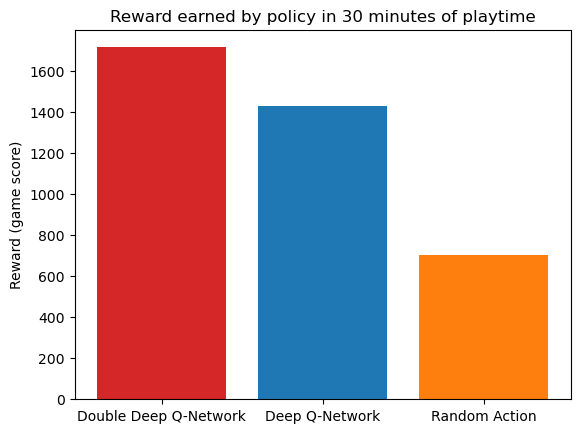
\includegraphics[width=1\linewidth]{Untitled.png}

\label{fig:4}
\end{figure}
While the double Q-network outperforms the regular Q-network, I wanted to see how they would compare when given a set amount of games to play instead of a set amount of time. Here each agent was given 1 game to earn as much reward as possible, averaged over 100 playthroughs. \newpage
\begin{figure}[h]
\centering
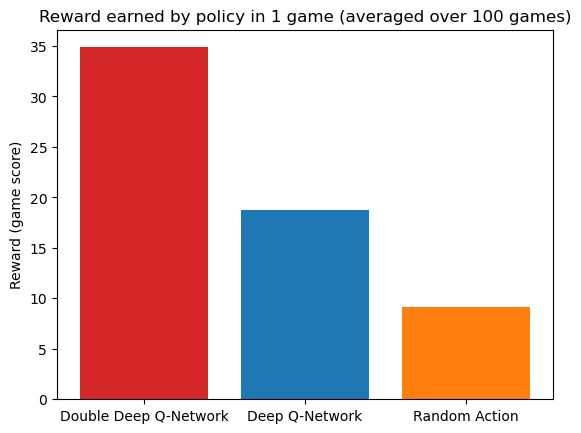
\includegraphics[width=1\linewidth]{Untitled2.png}

\label{fig:5}
\end{figure}
Here the double Q-network performs better than before.
My hypothesis is that a more aggressive policy can score you more points over a period of time,
but the less overoptimistic double Q-network is better at longevity and maximizing rewards while preserving limited lives. \par
In addition to quantitative data, I used Gymnasium's \texttt{rendering = 'human'} parameter to see what each network was doing. Here I noticed the issue where \texttt{noop_max} seemed not to be working, as the network was doing the exact same thing every time when sticky actions were turned off, which is what we would expect from a deterministic environment.
When I made \texttt{noop_max} much larger (\texttt{noop_max = 500}), I found that the agent was no longer acting deterministically. As such further training could likely be improved with a larger \texttt{noop_max} value.
In addition, I noticed that the agent seems to walk into the trucks on the road purposefully, whereas it avoids the other cars.  
My hypothesis is that the agent is confused by the color of the trucks being the same as the color of the frog you can rescue, which can reward points;  
this is questionable, however, as the points are only awarded when Frogger reaches a home bay, so the network shouldn't know the white frog awards points (as it never makes it to the home bay in my observations). If you would like to watch the model play Frogger yourself, you can load any of the provided models or train one yourself and use the observation environment at the end of the Jupyter notebook.
\newpage
\section{Conclusions and Further Research}
While the double Q-network outperformed the regular Q-network, there is a possibility that a regular Q-network with parameters tuned for it would provide a fairer comparison. A lack of foresight on my part caused the rewards at each saving to be lost, so I couldn't show how training progressed over time; future researchers should take care to save such data. Qualitatively from watching the training, rewards earned at each saving had high variance and capped at out 39 points in one playthrough, but there was a positive trend in rewards over time. On the other hand, the regular Q-network produced high variance results without even showing a positive trend; the best regular Q-network was saved in the first $1,000,000$ or so steps over around $30,000,000$ steps. Various improvements have been suggested throughout this paper, but there are some larger changes one could make to improve agent performance. A double expected SARSA network might be capable of outperforming a double Q-network. Parameters could be further tuned, and longer training times with a larger network could also improve performance. Temporal logic is very important in Atari games in general and Frogger specifically, as agents need to predict the trajectory of moving hazards in order to avoid them correctly. As such, using an attention mechanism akin to that used in transformer networks restructured for image input for Atari learning would be an interesting experiment that might improve performance.
\newpage
\printbibliography

\end{document}